%*************************************************
\chapter{Redes neuronales artificiales}\label{ch:NNBasics}
% ************************************************
\section{Introducción}

En el capítulo anterior se abordaron conceptos básicos del aprendizaje automático, así como dos de sus principales enfoques: aprendizaje supervisado y no supervisado. Las redes neuronales artificiales o \acs{ANN}s por sus siglas en inglés, son comúnmente un método de aprendizaje supervisado\footnote{Las redes neuronales artificiales son algoritmos que también se pueden aplicar en métodos de aprendizaje no supervisado.}, que han tenido gran impulso en los últimos años debido al incremento de datos y a su fácil acceso, así como al crecimiento en poder computacional.
\\
\\
Las \textbf{redes neuronales artificiales}  son algoritmos de aprendizaje automático que simulan\footnote{Las redes neuronales artificiales a menudo son consideradas más como una caricatura de las biológicas, pues su complejidad rebasa el entendimiento e interpretación que se le puede dar a través de los modelos de \acs{ANN}s.} el mecanismo de aprendizaje de los organismos biológicos, en donde las neuronas, es decir, las células del sistema nervioso, se conectan unas con otras mediante las dendritas y los axones en la región espacial nombrada sinapsis \autoref{fig:biologicalnn}, en donde las conexiones sinápticas a menudo cambian en respuesta a estímulos externos del organismo, proceso que a grandes rasgos es como aprenden los seres vivos. \cite{Nielsen:2018}

\begin{figure}[hb]
  \centering
  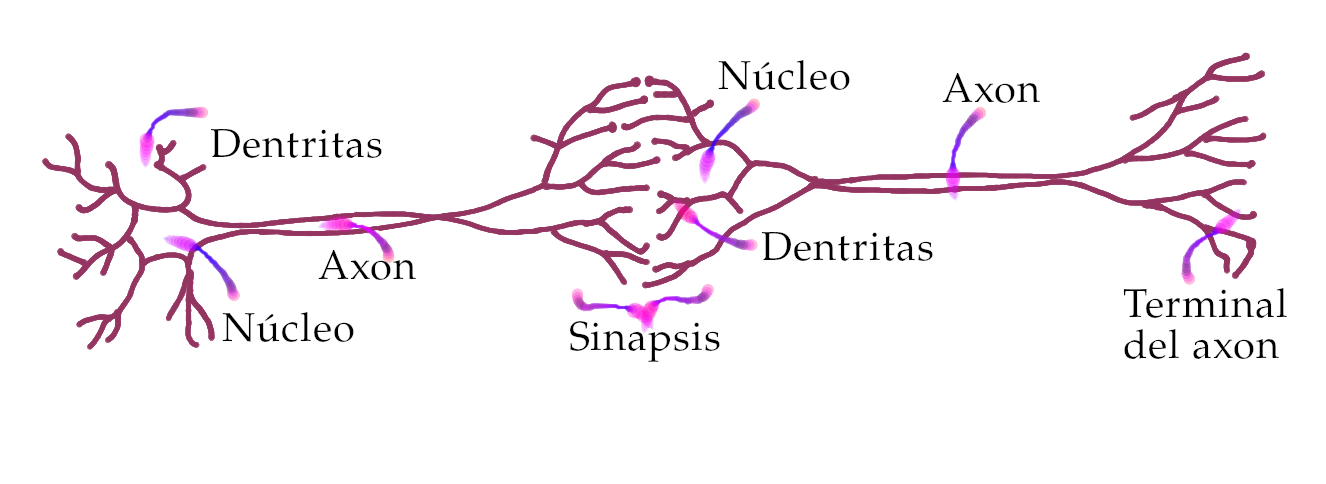
\includegraphics[width=0.75\textwidth]{./img/BioloNN.png}
  \caption{Neuronas biológicas transmitiendo información \cite{Gardell:2010}}
  \label{fig:biologicalnn}
\end{figure}


\section{Arquitectura básica}

\subsection{El perceptrón}\label{sec:perceptron}

La \autoref{fig:perceptron} muestra un diagrama de un modelo de perceptrón, que es el modelo más simple de las \acs{ANN}s. En este ejemplo la \textbf{capa de entrada}, o \textbf{input layer} en inglés, tiene dos componentes:
$$(x_1,x_2)$$
Es decir, $d=2$ en la \autoref{eq:trainset}. La constante $1$ es añadida para asignarle el \textbf{sesgo} o \textbf{bias} en inglés, denotado por: $b \in \mathbb{R}$, un parámetro que a menudo se emplea por razones de estadística. La \textbf{neurona}, \textbf{nodo}, o \textbf{node} en inglés, es la unidad computacional que calcula:

\begin{equation}
  \label{eq:neuronfun}
  f\left( \sum_{i=1}^dw_i\cdot x_i + b \right)
\end{equation}

donde los $w_i \in \mathbb{R}$ son conocidos como los \textbf{pesos}, o \textbf{weights} en inglés, de $x_i$, y $f$ es una función \autoref{sec:FuncAct}.
\begin{figure}[hb]
  \centering
  \begin{tikzpicture}[x=1.5cm, y=1.5cm]
    % Input nodes
  \node[circle, draw, fill=CTtitle!30] (vac) at (0,1) {$1$};
  
  \node[circle, draw, fill=CTtitle!30] (input1) at (0,3) {$x_{1}$};
  \node[circle, draw, fill=CTtitle!30] (input2) at (0,2) {$x_{2}$};
    
    % Summation node
  \node[circle, draw, fill=CTtitle!60, minimum size=1.5cm] (sum) at (2,2) {$\Sigma / f(\Sigma)$};
  % Activation node
  %\node[circle, draw, fill=CTtitle!60, minimum size=1.5cm] (activation) at (4,2) {$f(\Sigma)$};
  % Output node
  \node[circle, draw, fill=CTtitle!30] (output) at (4,2) {$\hat{y}$};
  % Connect the nodes and add weights
  \foreach \i in {1,2}
  \draw[->] (input\i) -- node[midway, above] {$w_{\i}$} (sum);
  \draw[->] (vac) -- node[midway, above] {$b$} (sum);
  %\draw[->] (sum) -- (activation);
  \draw[->] (sum) -- (output);

  \node[above, yshift=2.5cm] at (0,2) {Entrada};
  \node[above, yshift=2.5cm] at (2,2) {Neurona};
  \node[above, yshift=2.5cm] at (4,2) {Salida};
  
\end{tikzpicture}

\caption{Diagrama de un modelo simple de perceptrón}
\label{fig:perceptron}
\end{figure}

\marginpar{Para simplificar la lectura, en las siguientes secciones y capítulos se utilizará la palabra ``red'' para hacer referencia a la red neuronal artificial o \acs{ANN}.}El objetivo del algoritmo, es que mediante el entrenamiento de la red \autoref{sec:TrainNN} con un conjunto grande de $M$ datos: $\{\vec{x_j},y_j\}_{j=1}^{M}$ se obtengan los $w_i$ óptimos para que se cumpla:
$$y_l= \hat{y_l} = f\left( \sum_{i=1}^dw_i\cdot x_l \right)$$
con $y_l$ la etiqueta, o valor esperado, correspondiente al vector $\vec{x_l}$, en donde $(\vec{x_l},y_l)$ es un dato que no necesariamente pertenece al conjunto de entrenamiento que utilizó la red. Esta última propiedad es llamada \textbf{generalización del modelo}, y es lo que permite hacer predicciones sobre nuevos datos.

\subsection{Función de activación}\label{sec:FuncAct}

En la \autoref{eq:neuronfun} la función $f$ es conocida como una \textbf{función de activación} o \textbf{activation function} en inglés. Algunos ejemplos de funciones de activación comúnmente utilizadas se muestran en la \autoref{fig:examplesfuncact}. 

\begin{figure}[htbp]
\centering

\subfloat[$y=Tanh(x)$]{%
\begin{tikzpicture}[scale=0.7]
\begin{axis}[
    xmin=-4.5, xmax=4.5,
    ymin=-1.2, ymax=1.2,
    axis lines=middle,
    xtick={-4,-3,...,4},
    ytick={-1,-0.5,0.5,1},
    ticklabel style={font=\tiny},
    samples=200,
    domain=-4.5:4.5,
    every axis plot post/.append style={line width=1pt}
]
\addplot[CTurl] {tanh(x)};
\end{axis}
\end{tikzpicture}
\label{fig:tanh}
}
\hfill
\subfloat[$y=x$]{%
\begin{tikzpicture}[scale=0.7]
\begin{axis}[
    xmin=-4.5, xmax=4.5,
    ymin=-4.5, ymax=4.5,
    axis lines=middle,
    xtick={-4,-3,...,4},
    ytick={-4,-3,...,4},
    ticklabel style={font=\tiny},
    samples=200,
    domain=-4.5:4.5,
    every axis plot post/.append style={line width=1pt}
]
\addplot[CTurl] {x};
\end{axis}
\end{tikzpicture}
\label{fig:identity}
}

\subfloat[$y=ReLU$]{%
\begin{tikzpicture}[scale=0.7]
\begin{axis}[
    xmin=-4.5, xmax=4.5,
    ymin=-4.5, ymax=4.5,
    axis lines=middle,
    xtick={-4,-3,...,4},
    ytick={-4,-3,...,4},
    ticklabel style={font=\tiny},
    samples=200,
    domain=-4.5:4.5,
    every axis plot post/.append style={line width=1pt}
]
\addplot[CTurl] {max(0,x)};
\end{axis}
\end{tikzpicture}
\label{fig:ReLU}
}
\hfill
\subfloat[$y=Sign$]{%
\begin{tikzpicture}[scale=0.7]
\begin{axis}[
    xmin=-4.5, xmax=4.5,
    ymin=-4.5, ymax=4.5,
    axis lines=middle,
    xtick={-4,-3,...,4},
    ytick={-4,-3,...,41},
    ticklabel style={font=\tiny},
    samples=200,
    domain=-4.5:4.5,
    every axis plot post/.append style={line width=1pt}
]
\addplot[CTurl] {sign(x)};
\end{axis}
\end{tikzpicture}
\label{fig:sign}
}
\caption{Ejemplos de funciones de activación}
\label{fig:examplesfuncact}
\end{figure}

La importancia en la elección de una función de activación u otra es más notable en los siguientes casos:
\begin{enumerate}
\item En la capa de salida de cualquier modelo de red
\item En los modelos multicapa \autoref{sec:multicapamodels}
\end{enumerate}
En el primer caso, la función de activación está motivada por el tipo de valores que puede tomar la etiqueta $y$. En problemas de clasificación binaria, las funciones de activación comúnmente utilizadas son \emph{Tanh} o \emph{Sigmoid}, en problemas de clasificación múltiple la función \emph{Softmax}; cuando $y$ toma valores reales la función de activación utilizada es la \emph{Identidad} o \emph{Lineal} \autoref{fig:identity}.
\\
En el segundo caso, la importancia de elegir una función de activación no lineal entre capas para modelos de clasificación, por ejemplo, permite que el modelo pueda transformar un problema que inicialmente no es linealmente separable, a uno que sí lo es.


\subsection{Función de pérdida}
La \textbf{función de pérdida}, o \textbf{loss function} en inglés: $L(\hat{y},y)$ es la función que compara el resultado o salida de la red: $\hat{y}$ respecto a la etiqueta original $y$ correspondiente a la entrada $\vec{x}$, en otras palabras, indica qué tan bueno es el modelo implementado. El modelo es mejor cuanto menos sea la diferencia entre el valor predicho $\hat{y}$ respecto al valor esperado $y$.
\\
En el entrenamiento de una red, el objetivo es minimizar esta función a través de la actualización de los pesos $w_i$. La elección de la función de pérdida, depende del problema a resolver, como en el caso de la función de activación de la última capa. Para modelos en donde los valores de la salida $\hat{y}$ son reales, se puede utilizar una \emph{función de pérdida cuadrática} o \emph{mean square error (MSE)} en inglés:
\begin{equation}
  \label{eq:MSE}
  L = (\hat{y}-y)^2
\end{equation}

Para problema de clasificación binaria se puede utilizar:
\begin{equation}
  \label{eq:bin}
  L = log(1 + \exp(−y\cdot \hat{y}))
\end{equation}

mientras que para problemas de múltiples categorías, donde $\hat{y}=(\hat{y}_1, ..., \hat{y}_k)$ son las probabilidades\footnote{Las probabilidades de cada clase se pueden obtener aplicando la función de activación \emph{Softmax}.} de las $k$ clases\footnote{Las \textbf{clases} se refieren a las diferentes opciones de salida que puede tener una red de un problema de clasificación múltiple, por ejemplo si la red reconoce tres tipos de fruta, cada fruta es una clase distinta.} una función de pérdida que se puede aplicar es:
\begin{equation}
  \label{eq:otro}
  L = −log(\hat{y}_r)
\end{equation}
con $r$ la clase a la que corresponde la etiqueta $y$.

\subsection{Modelos multicapa}\label{sec:multicapamodels}
En la sección \autoref{sec:perceptron} se revisó el perceptrón como el modelo de red más simple. La \autoref{fig:nnlayers} muestra un diagrama de un modelo multicapa, estos modelos tienen capas ocultas entre las capas de entrada y salida, cada capa contiene un número determinado de neuronas o nodos. El número de capas ocultas y los nodos en cada una, son \textbf{hiper-parámetros} de la red, y en general\footnote{\emph{Hyperparameter grid search} es un método que se puede utilizar para conocer los hiper-parámetros óptimos de un modelo en particular, sin embargo, este proceso generalmente implica costos computacionales mayores.}, no se tiene una manera determinista para conocer los valores óptimos en cada modelo.

\begin{figure}[ht]
    \centering
    \begin{tikzpicture}[scale=1.5]
    
    % Input layer
    \foreach \i in {1,...,4}
        \node[circle, draw=black, fill=CTtitle!30] (I-\i) at (0,\i-2) {$x_{\i}$};
    
    % Hidden layer 1
    \foreach \i in {1,...,3}
        \node[circle, draw=black, fill=CTtitle!60] (H1-\i) at (2,\i-1.5) {};
    
    % Hidden layer 2
    \foreach \i in {1,...,3}
        \node[circle, draw=black, fill=CTtitle!60] (H2-\i) at (4,\i-1.5) {};
        
    % Output layer
    \foreach \i in {1,...,2}
        \node[circle, draw=black, fill=CTtitle!30] (O-\i) at (6,\i-1) {$y_{\i}$};
    
    % Connections
    \foreach \i in {1,...,4}
        \foreach \j in {1,...,3}
            \draw[->] (I-\i) -- (H1-\j);
            
    \foreach \i in {1,...,3}
        \foreach \j in {1,...,3}
            \draw[->] (H1-\i) -- (H2-\j);
            
    \foreach \i in {1,...,3}
        \foreach \j in {1,...,2}
            \draw[->] (H2-\i) -- (O-\j);
    
    % Labels
    \node[above, yshift=0.5cm] at (0,2) {Capa de Entrada};
    \node[above, yshift=0.5cm] at (2,2) {Capa oculta 1};
    \node[above, yshift=0.5cm] at (4,2) {Capa oculta 2};
    \node[above, yshift=0.5cm] at (6,2) {Capa de Salida};
    
    \end{tikzpicture}
    \caption{Diagrama de un modelo de \acs{ANN} multicapa con dos capas ocultas.}
    \label{fig:nnlayers}
\end{figure}

La arquitectura específica de las redes multicapa se conoce como redes \emph{feed-forward} en inglés, pues las capas se alimentan una tras otra desde la capa de entrada hasta la capa de salida. La arquitectura por defecto de las redes feed-forward supone que todos los nodos de una capa están conectados a los de la capa siguiente. \cite{Nielsen:2018}
\\
La operación que realiza una red multicapa de la capa de entrada a la primer capa oculta con $p_1$ nodos está definida como:
$$\vec{h}_1 = f(W^T_1 \cdot \vec{x})$$
onde $W^T_1$ es la transpuesta de $W_1$, de dimensión $p_1 \times d$, y $\vec{x}$ el vector de entrada de dimensión $d$. La operación que se realiza de la capa oculta $p$ a la $p+1$ $\forall p \in \{1,...,k-1\}$ es:
$$\vec{h}_{p+1} = f(W^T_{p} \cdot \vec{h}_p)$$
donde $W^T_{p}$ es de dimensión $p_{r+1} \times p_r$ y $\vec{h}_p$ es de dimensión $p$. Finalmente, de la última capa oculta a la capa de salida con dimensión $o$ la operación realizada es:
$$\vec{o} = f(W^T_{k+1} \cdot \vec{h}_k)$$
con $W^T_{k+1}$ de dimensión $o \times p_{k}$, y $\vec{h}_k$ de dimensión $p_k$. En todas las expresiones $f$ es una función de activación que se aplica a cada elemento del vector.

\section{Entrenamiento de una red neuronal}\label{sec:TrainNN}
Una vez construida la arquitectura de una red, el objetivo es obtener los parámetros $w$ y $b$ de cada nodo y en cada capa que minimicen la función de pérdida $L$. El algoritmo que se utiliza para minimizar la función de pérdida es conocido como \textbf{descenso del gradiente estocástico} o SGD por sus siglas en inglés. La \autoref{fig:gd} muestra un sencillo ejemplo del funcionamiento del algoritmo, en donde la función de pérdida únicamente depende de un parámetro $w$, el peso inicial es un valor aleatorio $w_1$, luego se calcula el valor del gradiente (en este caso unidimensional: la derivada) y se actualiza el peso como:
$$w_2 = w_1 - \alpha \frac{dL}{dw}\bigg|_{w_1}$$
en donde $\alpha$ es un hiper-parámetro de la red llamado \textbf{tasa de aprendizaje} o \textbf{learning rate} en inglés. El proceso continúa actualizando $w$ hasta llegar a $w_m$, el mínimo de la función de pérdida, pues el algoritmo actualiza los pesos en dirección opuesta al gradiente, que apunta a la dirección de máximo cambio.

\begin{figure}[h]
  \centering
  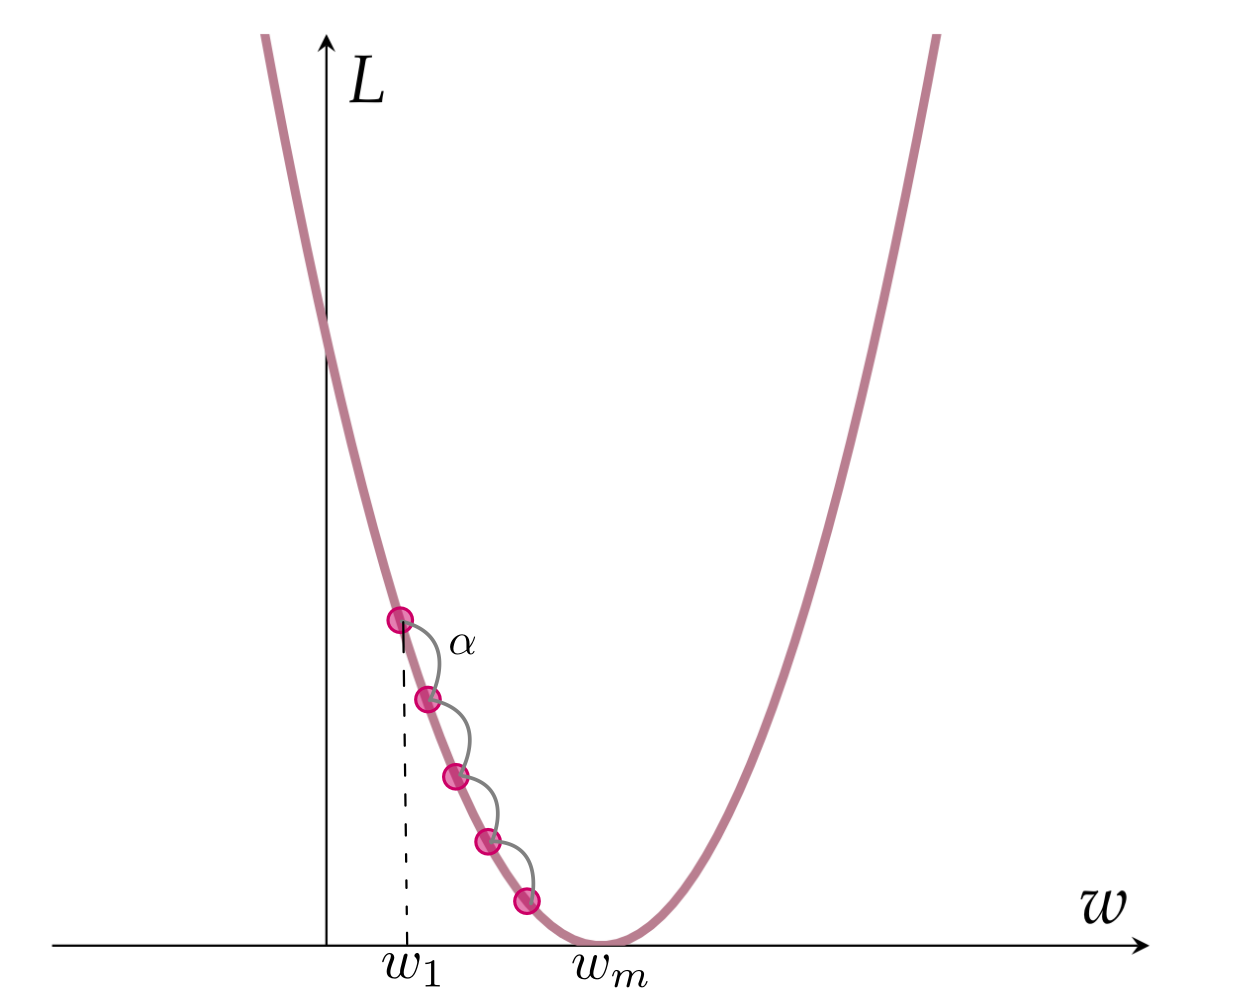
\includegraphics[width=0.7\textwidth]{./img/GD.png}
\caption{Algoritmo de descenso del gradiente para una función de pérdida $L(w)$}
\label{fig:gd}
\end{figure}

Para modelos de una capa el proceso del descenso del gradiente es directo, pues la función de pérdida depende de los pesos de la
única capa, sin embargo, para modelos multicapa la función de pérdida es el resultado de una composición de múltiples funciones de los pesos de las capas anteriores, el algoritmo utilizado para calcular el gradiente en función de la composición se llama \textbf{retropropagación} o \textbf{backpropagation} en inglés, que se compone de dos fases principales:
\begin{enumerate}
\item Fase de avance: La red recibe las entradas con pesos establecidos de manera aleatoria, se calcula la función de pérdida y las derivadas respecto a la última capa, es decir, la capa de salida.
  \item Fase hacia atrás: En esta fase el objetivo es conocer el gradiente de la función de pérdida respecto a los pesos de las capas anteriores utilizando la regla de la cadena.
\end{enumerate}

La \autoref{fig:backprop} muestra un ejemplo de la composición de funciones que se realizan en una red neuronal. En este ejemplo existen dos capas antes de la salida $o$.

\begin{figure}[h]
  \centering
  \begin{tikzpicture}[scale=0.7,x=2cm,y=2cm]
  \node[draw, circle, fill=CTtitle!30, minimum size=1.5cm] (x1) at (0,0) {$f(w)$};
  \node[draw, circle, fill=CTtitle!30, minimum size=1.5cm] (h1) at (2,1) {$g(y)$};
  \node[draw, circle, fill=CTtitle!30, minimum size=1.5cm] (h2) at (2,-1) {$h(z)$};
  \node[draw, circle, fill=CTtitle!30, minimum size=1.5cm] (y) at (4,0) {$K(p,q)$};
  
  \draw[->] (-1,0) -- (x1)node[midway, above left] {$w$};
  \draw[->] (x1) -- (h1) node[midway, above left] {$y=f(w)$};
  \draw[->] (x1) -- (h2) node[midway, below left] {$z=f(w)$};
  \draw[->] (h1) -- (y) node[midway, above right] {$p=g(y)$};
  \draw[->] (h2) -- (y) node[midway, below right] {$q=h(z)$};
  \draw[->] (y) -- (5,0) node[midway, above right] {$o=K(p,q)$};
\end{tikzpicture}
\caption{Gráfica computacional con dos posibles caminos \cite{Nielsen:2018}}
\label{fig:backprop}
\end{figure}

Utilizando la regla de la cadena para funciones de varias variables se puede determinar la derivada de $o$ respecto al peso $w$:

\begin{align}
  \label{eq:ugly}
\frac{\partial o}{\partial w} &= \frac{\partial o}{\partial p} \cdot \frac{\partial p}{\partial w} +  \frac{\partial o}{\partial q} \cdot \frac{\partial q}{\partial w}  \\ 
                              &=  \frac{\partial o}{\partial p}\cdot\frac{\partial p}{\partial y}\cdot\frac{\partial y}{\partial w} + \frac{\partial o}{\partial q}\cdot \frac{\partial q}{\partial z}\cdot \frac{\partial z}{\partial w}\\
                              &= \frac{\partial K(p,q)}{\partial p}\cdot g'(y)\cdot f'(w) + \frac{\partial K(p,q)}{\partial q}\cdot h'(z)\cdot f'(w)
\end{align}

En este ejemplo existen únicamente dos caminos posibles de $w$ a $o$. En la práctica, las redes neuronales multicapa contienen una gran cantidad de caminos posibles entre los pesos de cada capa hasta la salida. Si se considera una secuencia de capas ocultas: $h_1,...,h_k$ seguida de la capa de salida $o$ respecto a la cual se calcula la función de pérdida $L$, la parcial de la función de pérdida respecto al peso $w_{h_r, h_{r+1}}$ de la conexión de la capa $h_{r}$ a la capa $h_{r+1}$ es: \cite{Nielsen:2018}

\begin{equation}
  \label{eq:partialw}
  \frac{\partial L}{\partial w_{h_r, h_{r+1}}} = \frac{\partial L}{\partial o}\cdot \left( \sum_{(h_r,h_{r+1},...,h_k,o)\in \mathcal{P}}\frac{\partial o}{\partial h_k}\prod_{i=r}^{k-1}\frac{\partial h_{i+1}}{\partial h_i}\right) \frac{\partial h_r}{\partial w_{h_{r-1},h_r}}
\end{equation}

con $\mathcal{P}$ el conjunto de las capas ocultas. Una vez conocidos los gradientes respecto a los pesos en las múltiples capas, se actualizan los valores $w$ con el objetivo de minimizar la función de pérdida, y así mejorar el modelo.\\
El número de datos de entrenamiento, es decir de pares: $(X_l,y_l)$, que pasan por la red antes de que se actualicen los pesos, se llama \textbf{tamaño de lote} o \textbf{batch size} en inglés. Una vez que todos los datos de entrenamiento han pasado por la red, se dice que ha pasado una \textbf{época} o \textbf{epoch} en inglés. Tanto el número de épocas, como el tamaño de lote son hiper-parámetros de la red.

%K(p,q)=K(g(f(w)),h(f(w)))
